\documentclass[12pt]{article}

\usepackage{mathtools}
\usepackage{blindtext}

\usepackage[margin=1in]{geometry}

\newcommand*{\eu}{e}
\newcommand*{\iu}{i}

\DeclarePairedDelimiter{\bra}{\langle}{\rvert}
\DeclarePairedDelimiter{\ket}{\lvert}{\rangle}
\DeclarePairedDelimiterX{\braket}[2]{\langle}{\rangle}
  {#1\,\delimsize\vert\,\mathopen{}#2}

\usepackage{biblatex}
\addbibresource{report.bib}

\usepackage[hidelinks]{hyperref}

\title{Solving Decoherence Channels on Open Quantum Systems}
\author{David Basoco \and Jack Hetherington \and Davis Rash \and Tim Ross}
\date{November 8, 2023}

\begin{document}
  \maketitle

  \section{Introduction}
  No quantum system is perfectly isolated from the environment. The case for the closed quantum systems, where the equation of motion is fully describing the state dynamics is the Schr\"{o}dinger equation. Generally, the dynamics of open quantum systems are described by a master equation, usually Lindbladian. Only under certain assumptions, known as the Born-Markov approximation, one can get an equation in this form able to describe the physical evolution of the quantum states. When these assumptions are not satisfied, we enter the non-Markovian realm. This distinction and breakdown of equations in changing scope illustrates how the open quantum systems theories are far from being completely solved.  

  We will cover several test beds for experimental research into open quantum systems. These test bed classs include Depolarizing and Puali channels, Markovian Reservoir Engineering and Amplitude damping. These experimental results demonstrate the versatile nature of quantum simulators and how they can be used for verifying and exploration into open quantum physics. 
  \blindtext

  \section{Applications}
  As we continue to make quantum computers larger, we generate macro systems that begin to enter the classical realm. As these systems grow the natural decoherence of quantum phenomenon rapidly increases. This results in qunatum systems that rapidly decohere in the presence of the environment or other micro states. The range is vast for this field of inquiry. From solid state physics to quantum field theory, from quantum chemistry and biology to quantum thermodynamics, numerous fields stand to benefit from understanding how macro quantum states interact and form the classical regime we interact with daily.
  \blindtext

  \section{Depolarizing and Pauli Channels}
  The depolarizing channel was examined by first applying it on a stationary state ($\vert\psi_0\rangle = U(\frac{\pi}{4}, \frac{\pi}{4},0)\vert 0\rangle$), with increasing values for $p$ ($p$ being the probability of an error). It was shown that the system was decohering into an $\frac{I}{2}$ state as desired by plotting the real diagonal values and the real and imaginary of one of the off-diagonals. The real of the diagonal values both went to $\frac{1}{2}$ as $p$ increased, and both components of the off-diagonal went to 0, which shows that the state was progressing towards an $\frac{I}{2}$ state as intended. The density matrix was found by using the Qiskit tomography experiment. 

The depolarizing channel was examined further by applying it to an oscillating circuit and time evolving that circuit with increasing decay rates. The expectation value of the $\vert 0 \rangle$ state of the oscillating system was plotted over time. In all cases where the decay rate is greater than 0, the expectation value of $\vert 0 \rangle$ decohered to $\frac{1}{2}$ over time instead of continuing to oscillate, whereas the case where they decay rate was 0, the circuit continued to oscillate between 1 and 0. 

The Pauli Channel was examined by first starting a initializing a system and memory qubit in the Bell State $\vert \psi - \rangle$. The Pauli Channel was added to the circuit affecting the system qubit. This circuit was time evolved so the decoherence could be watched. The rate of decoherence was effected by the values: time, eta, and omega. These three values affect the probabilities of the three Pauli gates, and there are two different methods used to generate the probabilities of the gates from these parameters, the non-CP-divisible map and the eternally non-Markovian. The state of both the system and memory qubits was measured with the Qiskit Experiment Tomography Experiment, and the work extractable was calculated from that state. The extractable work was plotted over time for each of the two methods, which gave us a similar plot to the plot from the reference material.

  \section{Markovian Reservoir Engineering}
  \blindtext

  \section{Amplitude Damping}
  \blindtext

\section{Trace Distance}
        The goal for the trace distance, is to determine the difference between the expected result and the simulated noise result. We can use that the trace distance is half of the trace of the absolute value of the difference of the two density matrices. \\
        Qiskit allows you to obtain the density matrix for a given quantum circuit fairly easily. However it is impossible to obtain the density matrix for a measured set of results. But, we can obtain an approximate density matrix by calculating the probability of being in a specified state then creating an approximate wave function, which we can then use to create an approximate density matrix. From here we can calculate the trace distance.  

  \section{Results}
  \subsection{Trace Distance}
        We were unable to measure the trace distance for our given set of cases, for the reservoir engineering and depolarizing channel it was not possible to create a density matrix from the results that matched in dimension of the one generated by the circuit without affecting the results.

  \begin{figure}
    \centering
    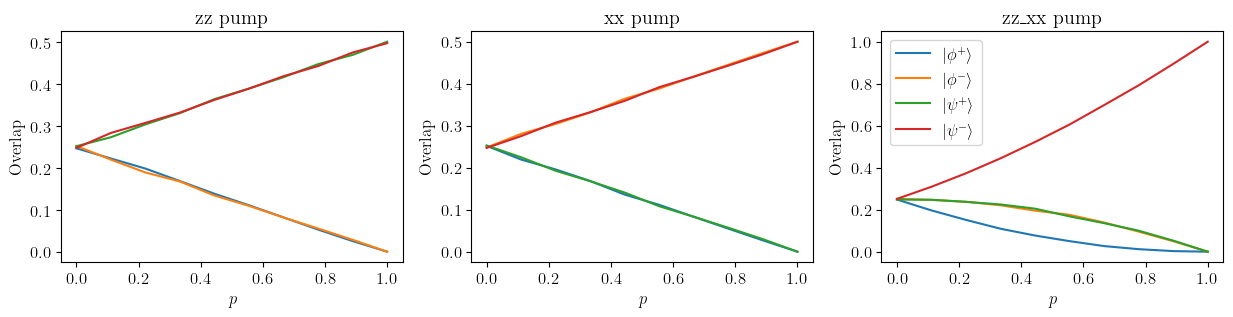
\includegraphics[width=\textwidth]{images/reservoir-engineering-simulation}
    \caption{Simulation of a quantum circuit.%
      \label{fig:reservoir-engineering-simulation}}
  \end{figure}

  \printbibliography
\end{document}